\section{Construcción}

\subsection{Modulo de carga y alimentación}

Dentro del sistema es critico el constante monitoreo de las variables de orientación,
temperatura y respiración del bebé, para ello se utilizó una pila Li-Po para mantener
alimentado el sistema. Al no poderse utilizar unicamente la batería de forma directa, se
diseño el siguiente modulo de carga y alimentación, el cual esta construido por 3 partes:

\begin{figure}[htp!]
    \centering
    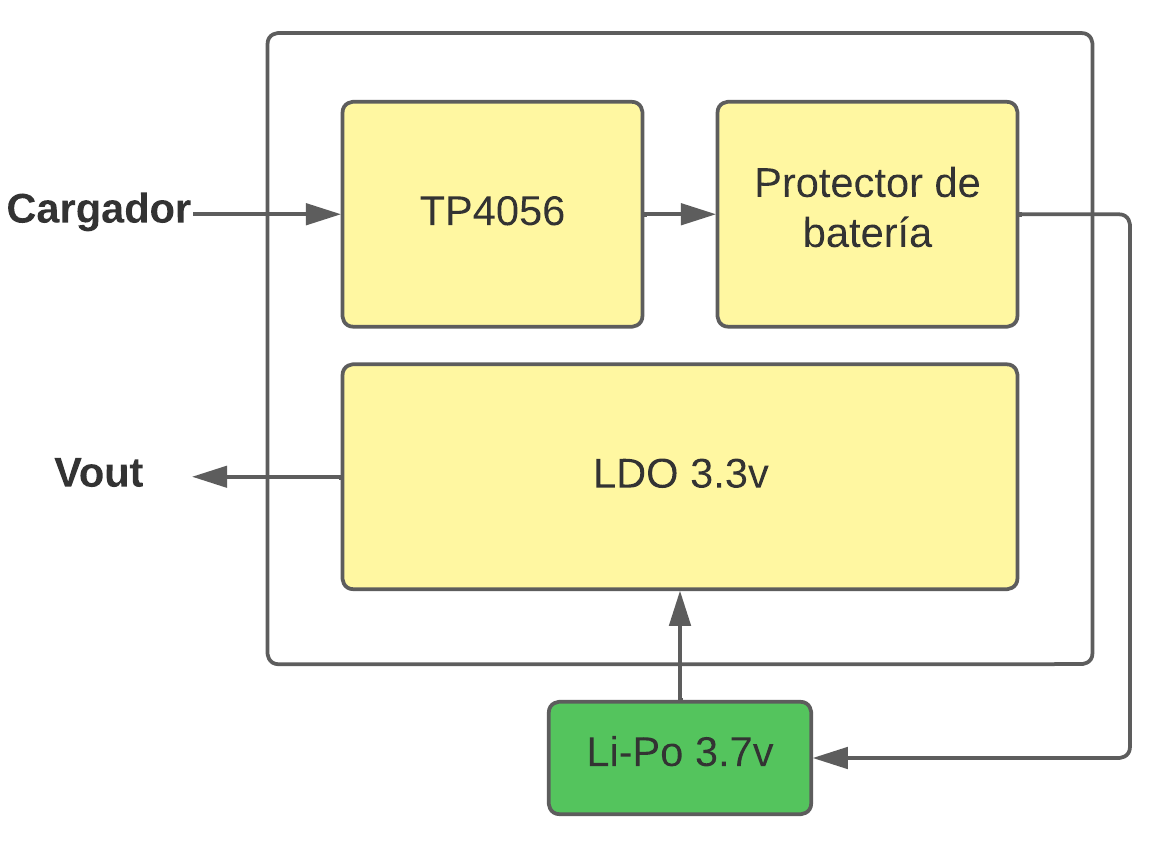
\includegraphics[width=\columnwidth]{charging_and_power_supply_module.png}
    \caption{Partes que conforman el modulo de carga y alimentación}
    \label{fig: charging_and_power_module}
\end{figure}
\FloatBarrier

\begin{figure}[htp!]
    \centering
    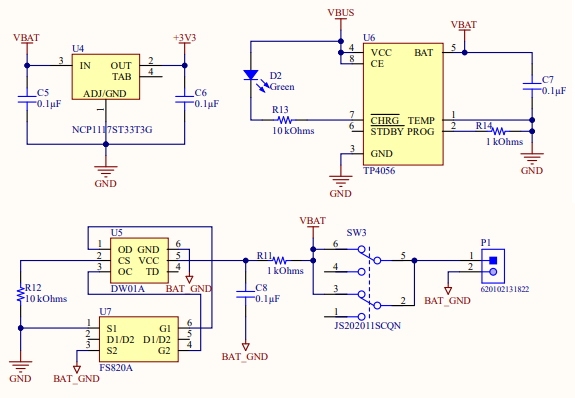
\includegraphics[width=\columnwidth]{battery_module_schematic.png}
    \caption{Esquematicos del modulo de carga y alimentación}
    \label{fig: battery_module_schematic}
\end{figure}
\FloatBarrier

\subsection{Diseño de PCB}

\subsubsection{Layout}
El diseño del PCB se realizo siguiendo una vision de obtener un dispositivo
minimo y pequeño para evitar incomodidades en el bebe.

A continuación se muestra el layout final de la primera versión:

\begin{figure}[htp!]
    \centering
    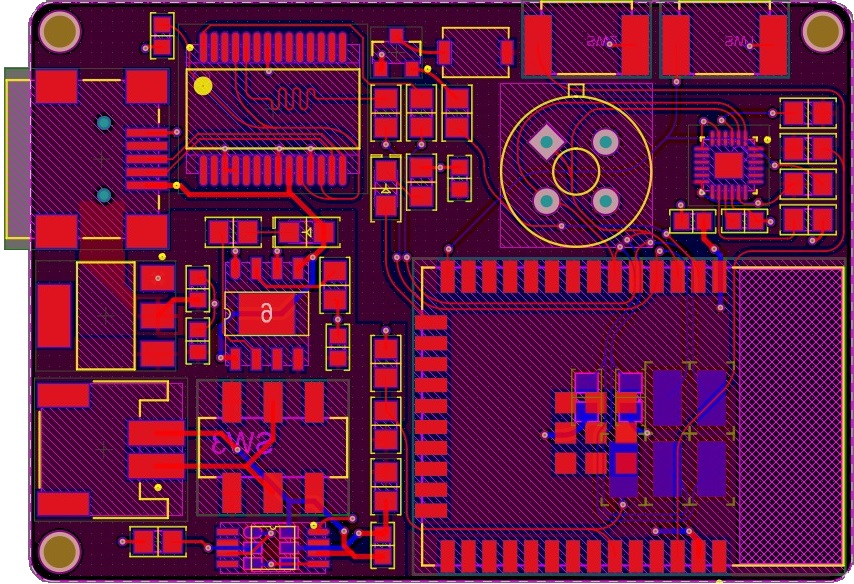
\includegraphics[width=\columnwidth]{layout.jpeg}
    \caption{Layout del PCB}
    \label{fig: layout}
\end{figure}
\FloatBarrier

\subsubsection{PCB 3D}
\begin{figure}[htp!]
    \centering
    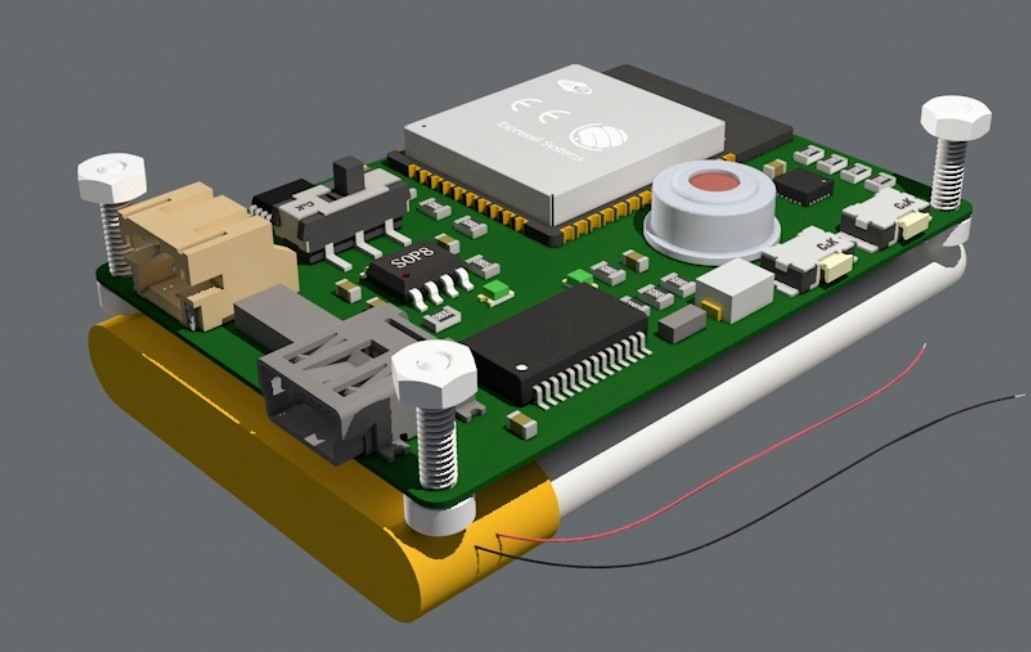
\includegraphics[width=\columnwidth]{isometric_view_3D.jpg}
    \caption{Vista isometrica del PCB y la batería}
    \label{fig: isometric_3d}
\end{figure}
\FloatBarrier
\begin{figure}[htp!]
    \centering
    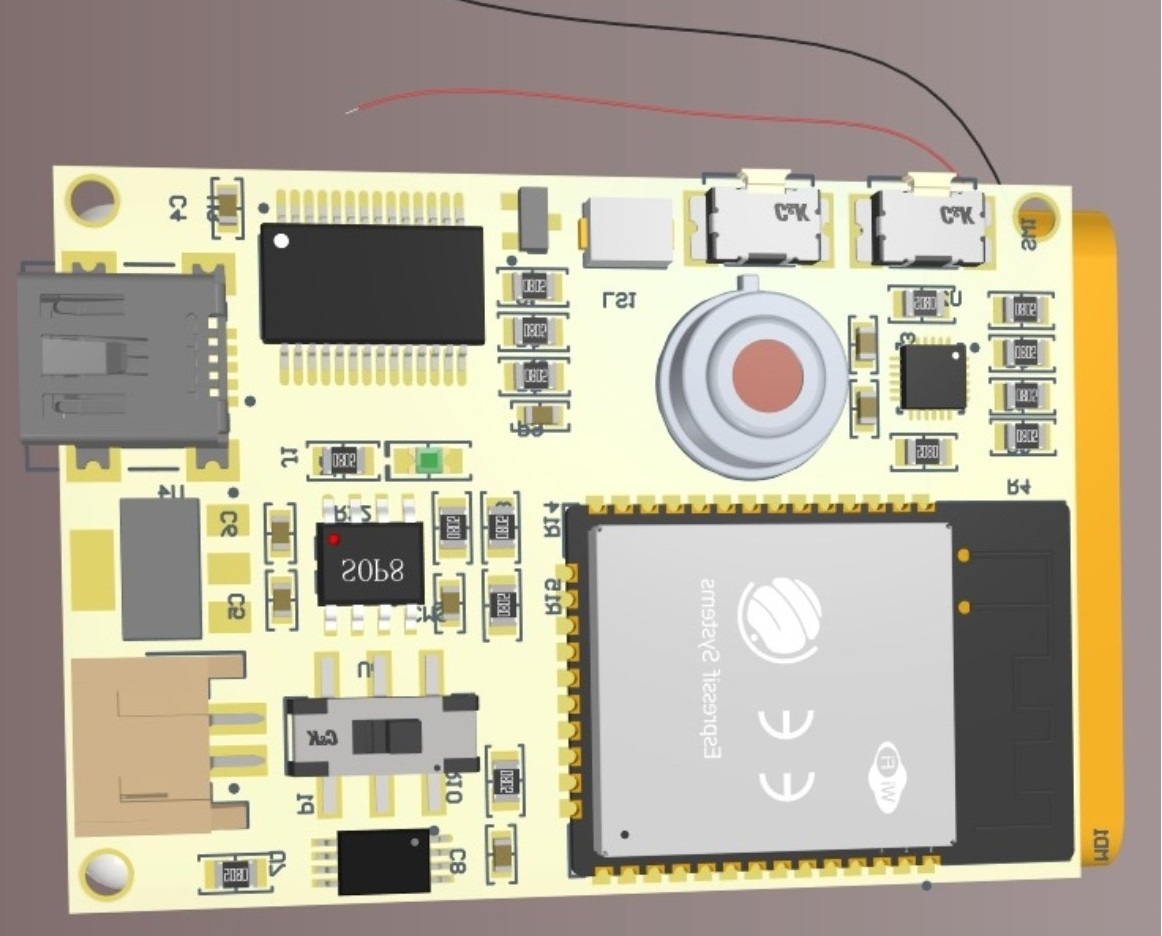
\includegraphics[width=\columnwidth]{top_view_3D_1.jpg}
    \caption{Vista superior del PCB}
    \label{fig: top_3d}
\end{figure}
\FloatBarrier

En las figuras \ref{fig: isometric_3d} y \ref{fig: top_3d} se muestra el modelo 3D, este fue hecho
para poder corraborar de que tamaño quedaría el dispositivo final contando la PCB y la batería.

Tanto el modelo 3D como el layout de la PCB fue diseñado en el software Altium.
\subsection{Diseño de Carcasa}
\begin{figure}[htp!]
    \centering
    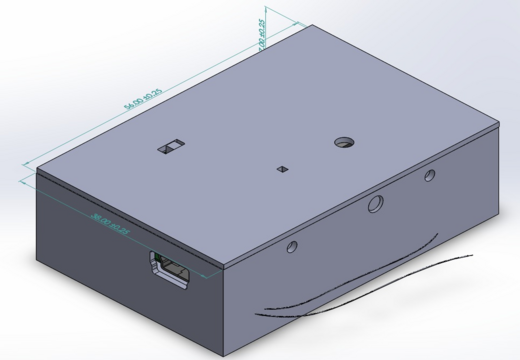
\includegraphics[width=\columnwidth]{system_shell_v2.png}
    \caption{Vista isometrica de la carcasa}
    \label{fig: isometric_view_shell}
\end{figure}
\FloatBarrier

\begin{figure}[htp!]
    \centering
    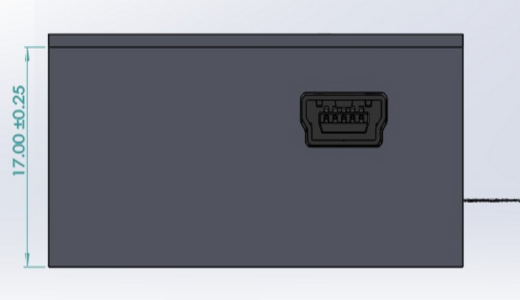
\includegraphics[width=\columnwidth]{front_view_system_shell_v2.png}
    \caption{Vista de la parte frontal de la carcasa, donde esta el puerto USB}
    \label{fig: front_view_shell}
\end{figure}
\FloatBarrier

\begin{figure}[htp!]
    \centering
    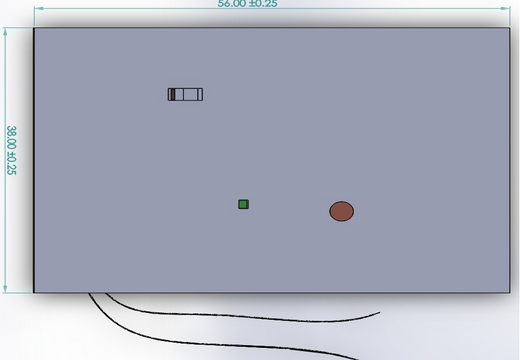
\includegraphics[width=\columnwidth]{top_view_syste_shell_v2.png}
    \caption{Vista superior de la carcasa}
    \label{fig: top_view_shell}
\end{figure}
\FloatBarrier

\begin{figure}[htp!]
    \centering
    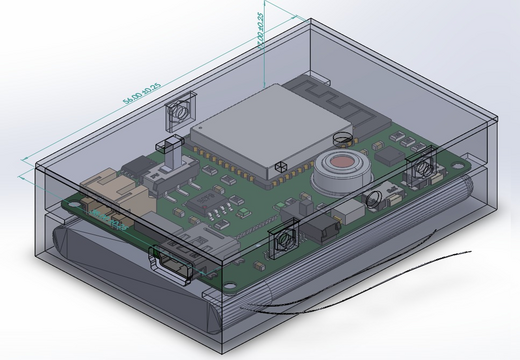
\includegraphics[width=\columnwidth]{system_shell v2_w_pcb.png}
    \caption{Vista isometrica de la carcasa con la PCB y bateria dentro}
    \label{isometric_view_pcb_shell}
\end{figure}
\FloatBarrier

En las figuras \ref{fig: isometric_view_shell}, \ref{fig: front_view_shell},
\ref{fig: top_view_shell} y \ref{isometric_view_pcb_shell}, se puede ver el diseño propuesto
para la carcasa del sistema, donde esta tendra las siguientes aberturas:

\begin{itemize}
    \item Switch encendido/apagado
    \item Puerto de carga Micro-USB tipo-B
    \item Salida para el sonido del buzzer
    \item Led infrarrojo del sensor de temperatura
\end{itemize}

